\chapter{Object Detection using Computer Vision}

\paragraph*{}
In the current simulation on Webots, the object detection system utilises OpenCV with a masking method to identify and interact with a yellow object in the arena. The task involves detecting and moving a yellow cylindrical object, randomly placed within the arena, to a specified location.

\paragraph*{}
The detection process commences with the robot utilising an RGB camera mounted on the front-most part of the TurtleBot3 to capture its surrounding environment. To address potential issues related to the robot's physics and balance, the RGB camera is approximated as a point source, as illustrated in Figure~\ref{fig:object detection figure 1}. The captured image is subsequently converted into the HSV colour space to facilitate the segmentation of the yellow object based on a predefined colour range. A mask is then applied to the regions containing the yellow colour, enabling the generation of a contour around the detected object. This contour functions as a visual boundary, allowing the robot to perceive and localise the object with precision.

\begin{figure}[H]
    \centering
    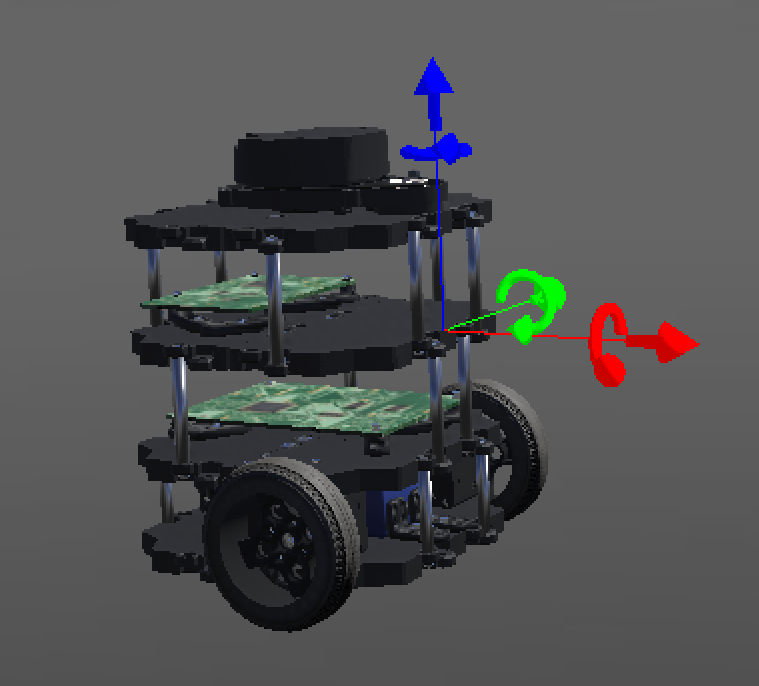
\includegraphics[width=0.5\linewidth]{assets/images/object_detection/fig1.png}
    \caption{The location of the RGB camera mounted on the TurtleBot3}
    \label{fig:object detection figure 1} 
\end{figure}

\paragraph*{}
Once the object is detected, the robot moves until the contour is centred within the camera frame, ensuring that the robot faces the object directly. This alignment is achieved by comparing the distances between the left and right edges of the bounding box surrounding the contour and the corresponding edges of the camera frame. Specifically, the distance between the left edge of the frame and the left edge of the bounding box is compared with the distance between the right edge of the frame and the right edge of the bounding box. The robot stops when the difference between these two distances is less than or equal to 1, as the camera calculates distances as whole numbers. Using a threshold of \(\leq 1\) is more reliable than requiring exact equality, as slight variations in measurement may occur due to the camera's resolution or other factors. See Figure \ref{fig:obj-flow}

\begin{figure}
    \centering
    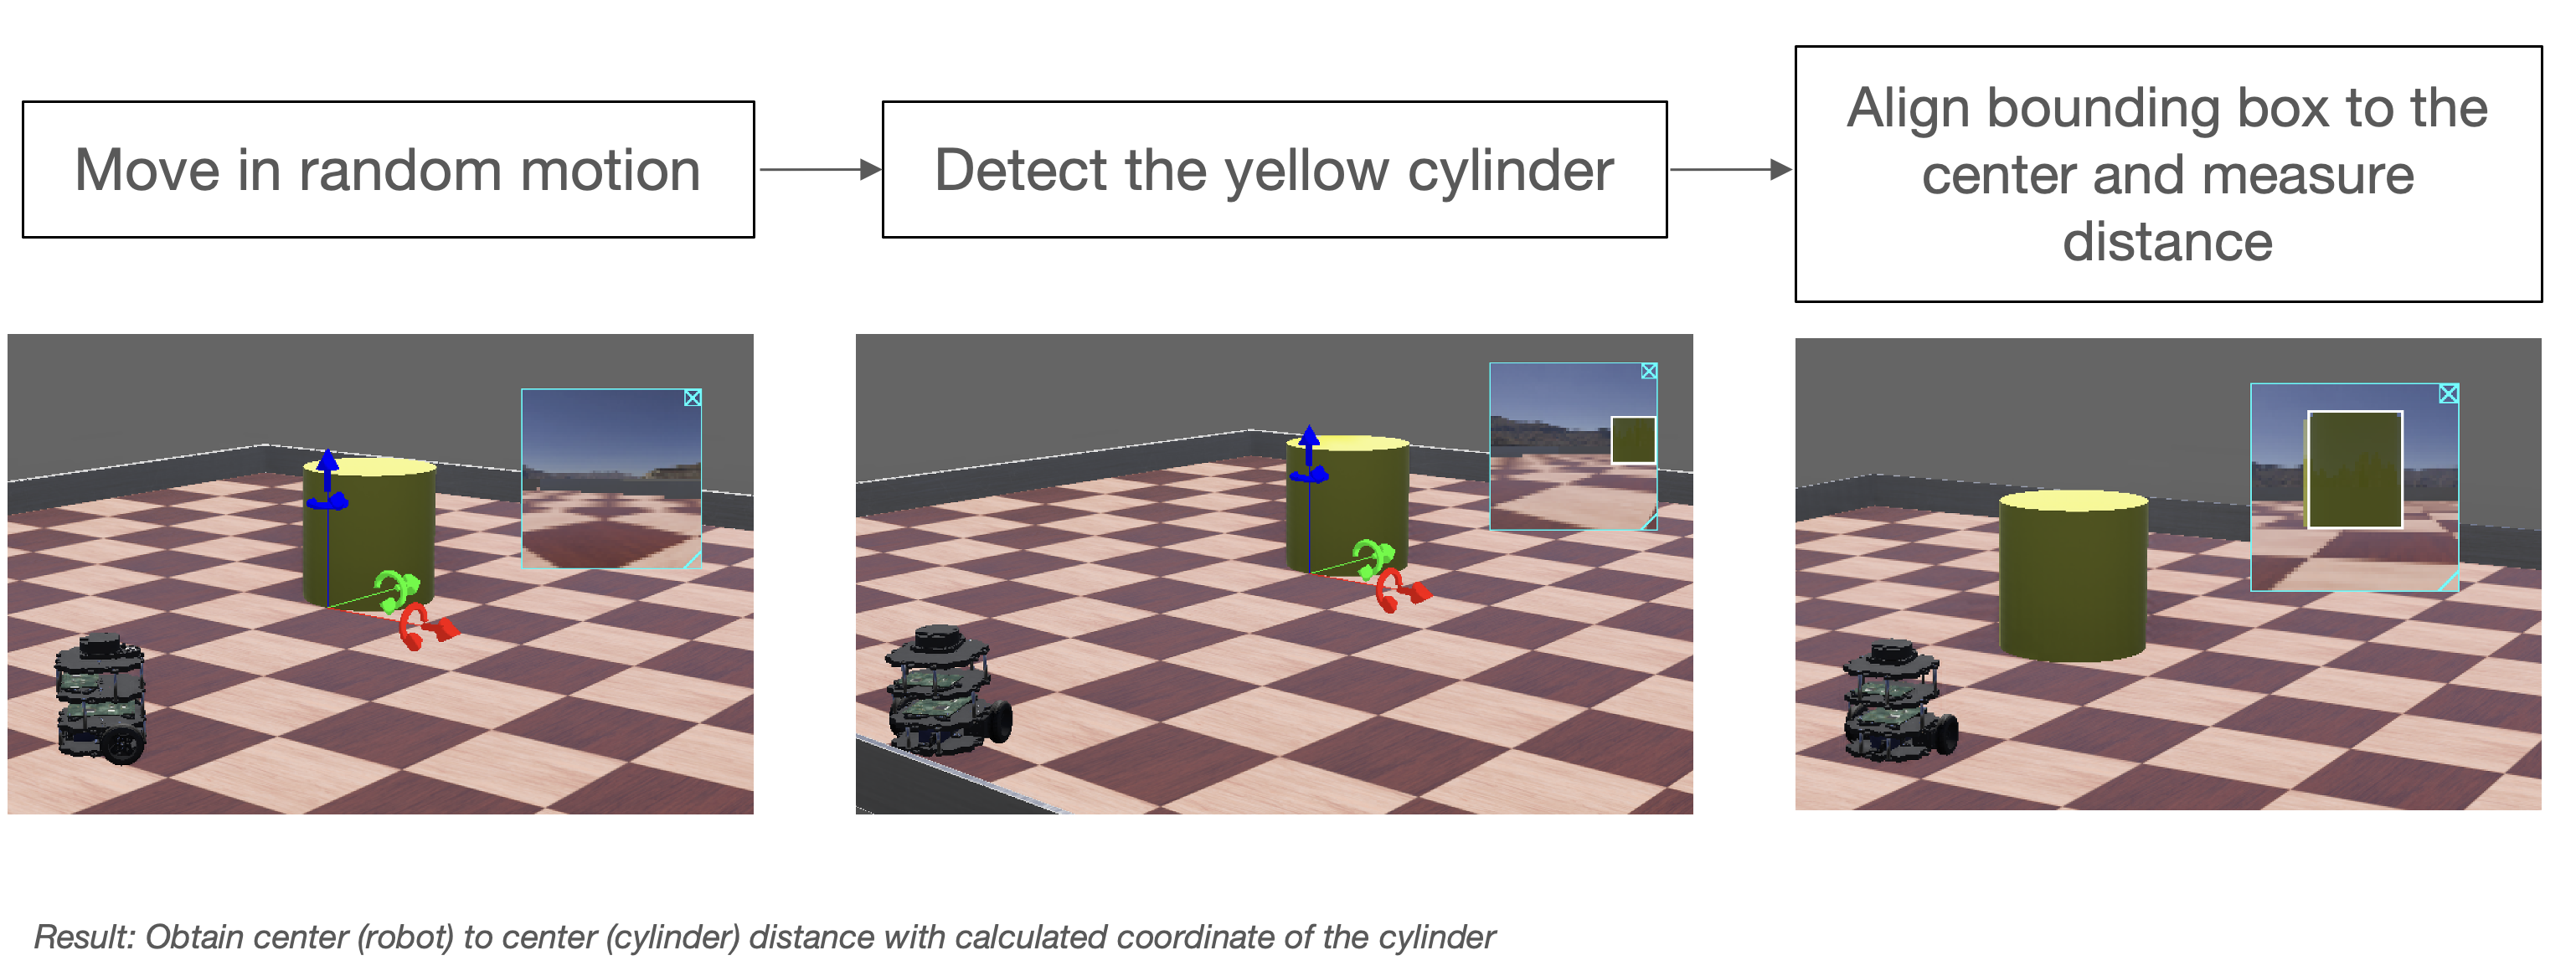
\includegraphics[width=0.8\linewidth]{assets/images/object_detection/obj-flow.png}
    \caption{Object Detection Flowchart}
    \label{fig:obj-flow}
\end{figure}

\begin{figure}[H]
    \centering
    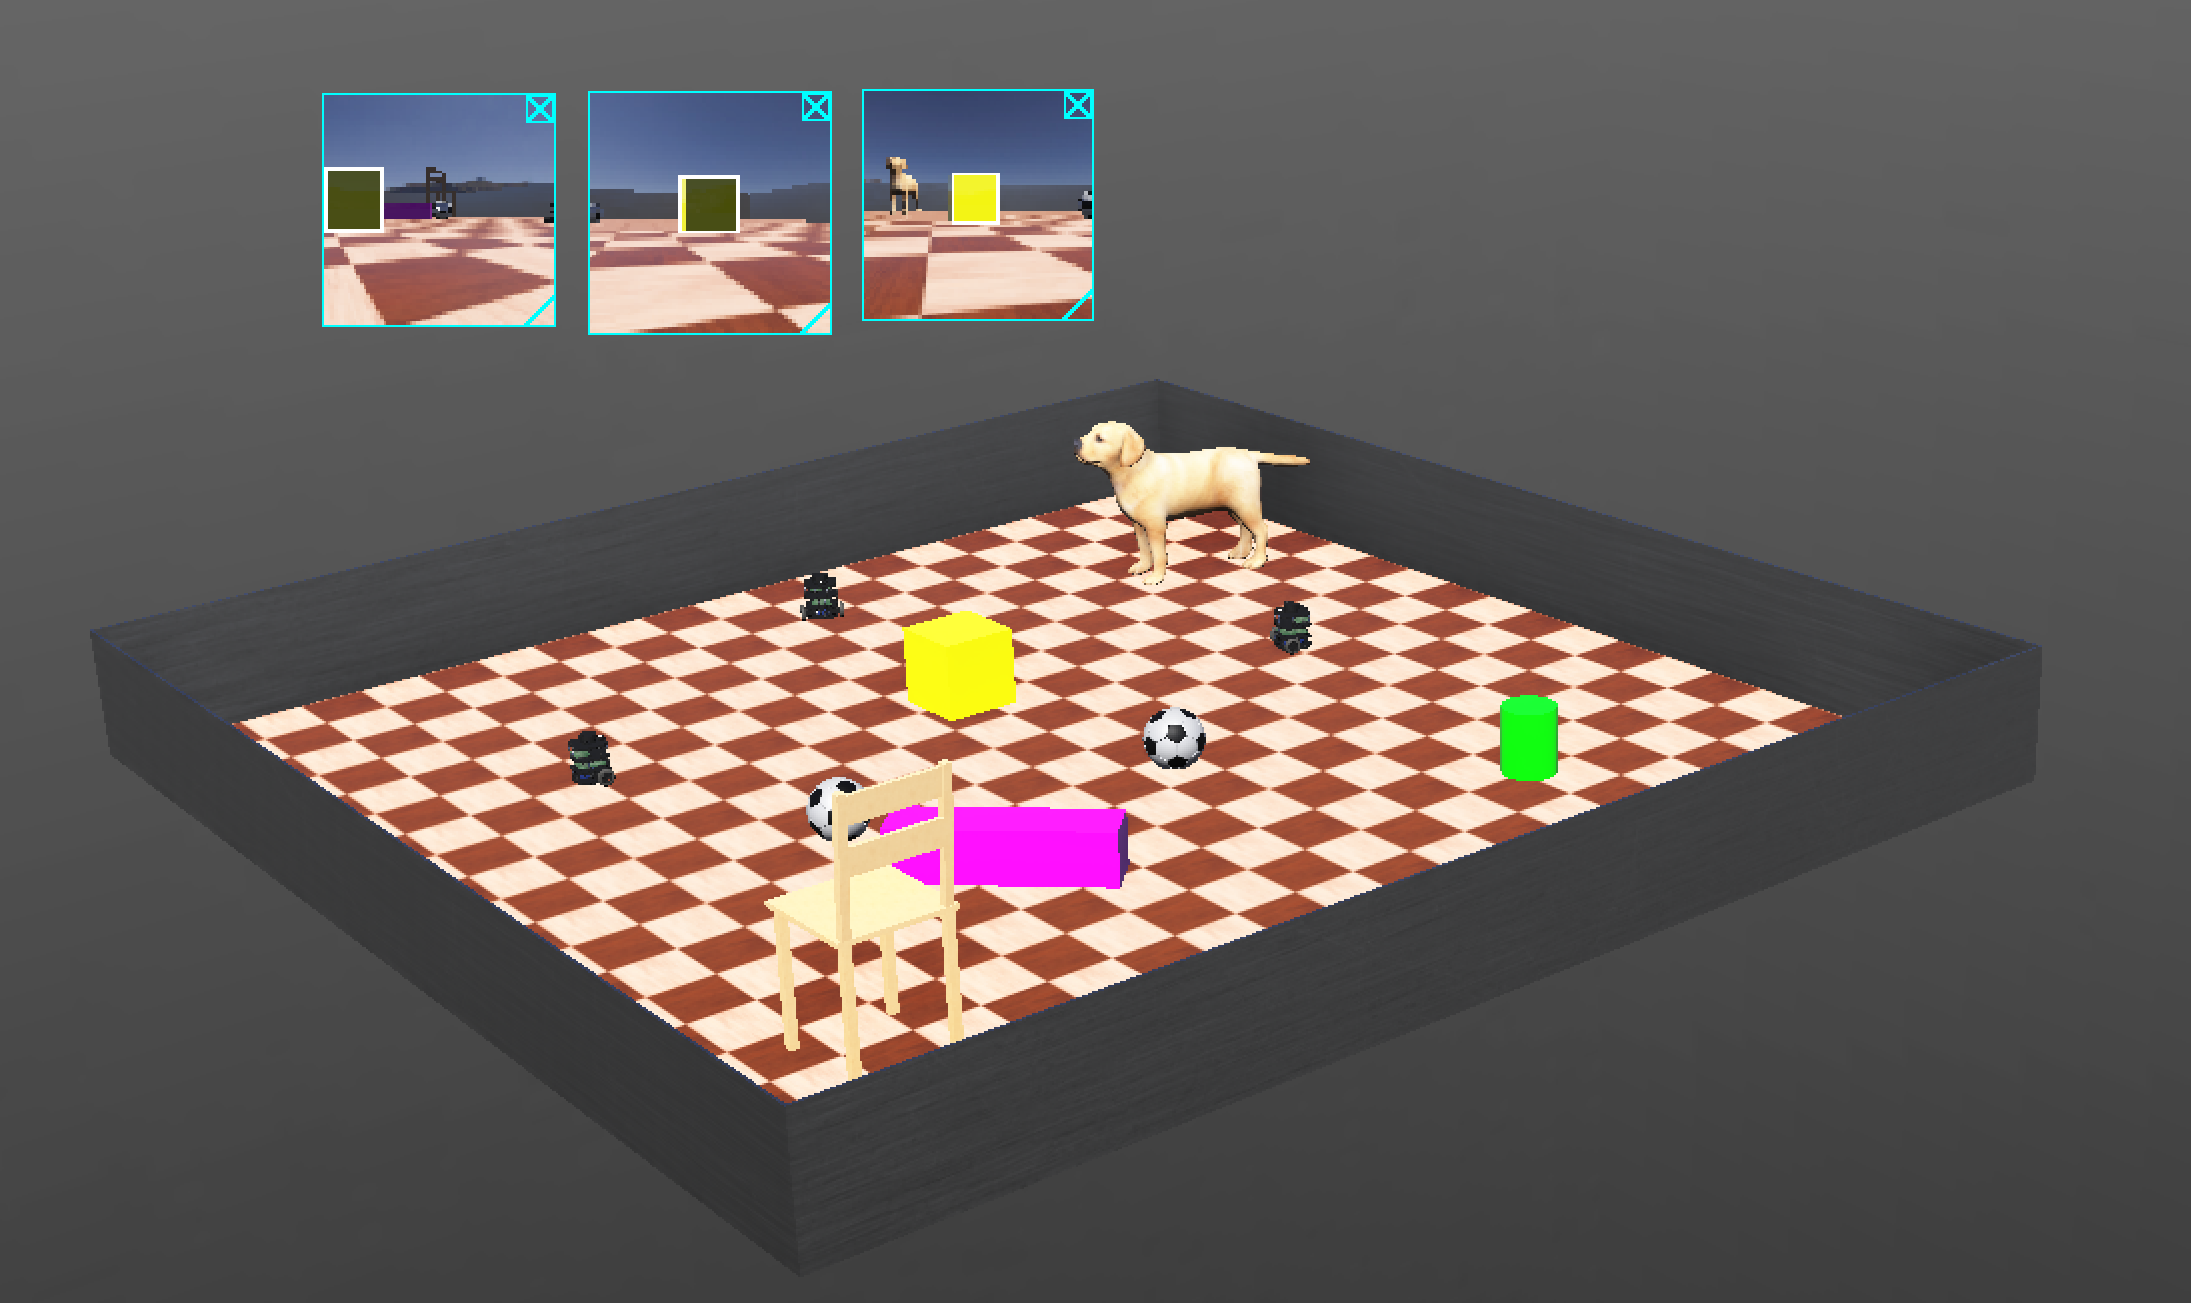
\includegraphics[width=1.0\linewidth]{assets/images/object_detection/fig2.png}
    \caption{The location of the RGB camera mounted on the TurtleBot3}
    \label{fig:object detection figure 2} 
\end{figure}

\paragraph*{}
After aligning with the object, as illustrated in Figure~\ref{fig:object detection figure 2}, the robot determines the real-world distance between its current position and the object's surface. By utilising the known distance and real-world dimensions of the object within the simulation, the system computes the real-time distance from the robot's camera to the object's surface. This information guides the robot in determining the distance it must travel to reach the yellow cylindrical object. The calculation is performed using a pre-determined focal length of the camera, derived through the following formulas:

\begin{equation}
\text{f} = \frac{H_{\text{real}}\cdot D_{\text{known}}}{H_{\text{img}}}\
\label{eq: focal length}
\end{equation}

\begin{equation}
\text d_{\text{real}} = \frac{H_{\text{real}}\cdot f}{H_{\text{img}}}\
\label{eq: real world distance}
\end{equation}

Where:
\begin{itemize}
    \item \( f \) represents the focal length of the camera (in pixels),
    \item \( H_{\text{img}} \) is the known width of the object in the image (in pixels),
    \item \( D_{\text{known}} \) denotes the known distance to the object (in metres),
    \item \( H_{\text{real}} \) is the real-world width of the object (in metres),
    \item \( f \) is the focal length of the camera (in pixels).
\end{itemize}

\paragraph*{}
To calculate the real-world distance, the process begins by determining the focal length of the camera. The positions of both the robot and the cylinder are defined within the simulation. The distance perpendicular to the outermost surface of the cylinder and the RGB camera mounted on the robot is denoted as \(D_{\text{known}}\). The cylinder's height in the real world, defined in the simulation, is represented as \(H_{\text{real}}\), while \(H_{\text{img}}\) corresponds to the detected height in pixels, obtained via the OpenCV model. Using Equation~\ref{eq: focal length}, the focal length \(f\) is calculated. This focal length is then applied in Equation~\ref{eq: real world distance}, along with \(H_{\text{real}}\), \(H_{\text{img}}\), and \(f\), to compute \(d_{\text{real}}\), the real-world distance. Once the real-world distance is obtained, we will add the radius of the target and the distance between the centre of the TurtleBot and the RGB camera so that we can get the distance from the centre of the robot to the centre of the target, which will be utilised further for determining the coordinate of the target on the map.

\paragraph*{}
The location of the target can be determined using data from the robot’s odometry, including its position (x, y) and orientation (yaw) relative to the origin (0, 0) of the map, as shown in Figure~\ref{fig:coordinate visualization}.

\begin{figure}[H]
    \centering
    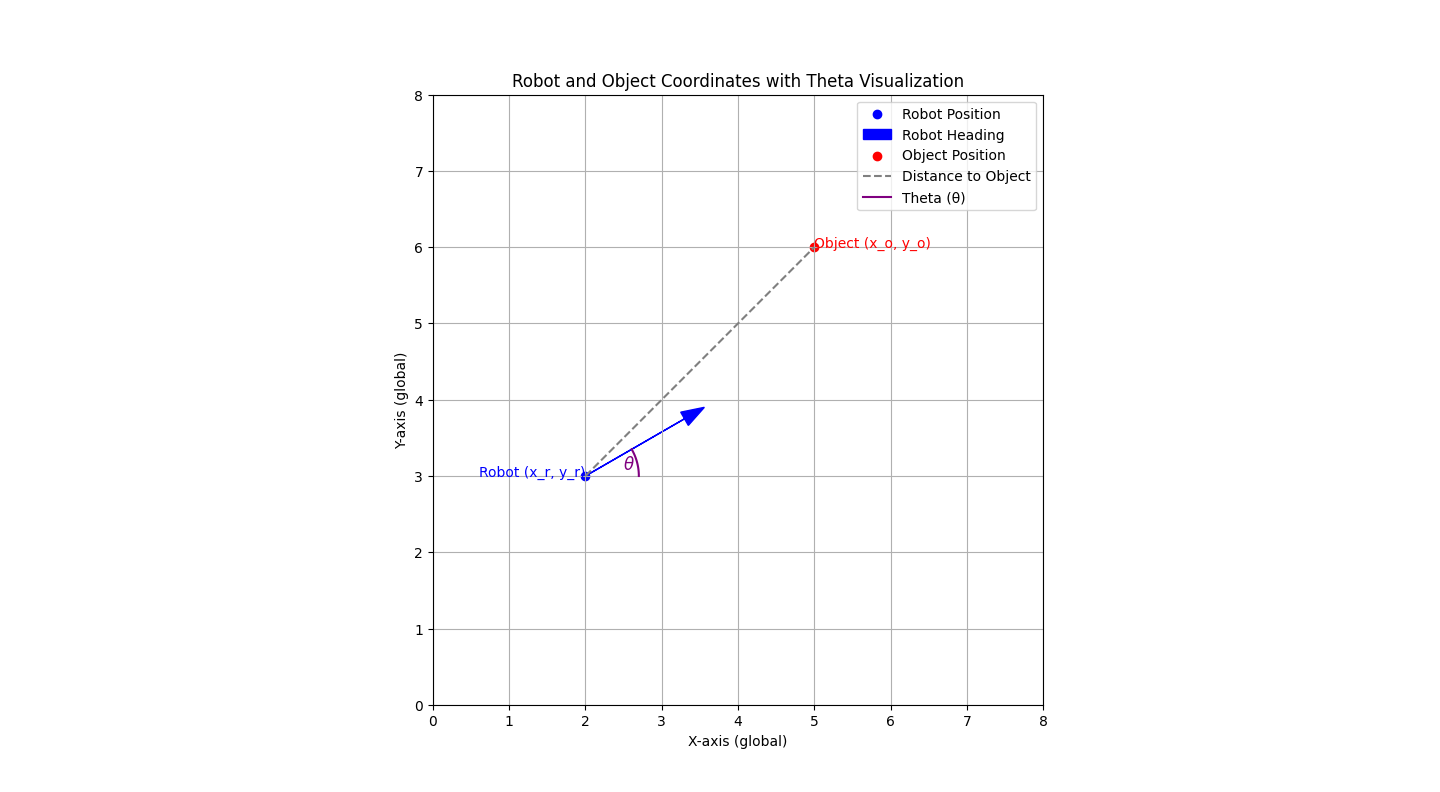
\includegraphics[width=1.1\linewidth]{assets/images/object_detection/fig3.png}
    \caption{The location of the RGB camera mounted on the TurtleBot3}
    \label{fig:coordinate visualization} 
\end{figure}

\paragraph*{}
By applying trigonometry, the coordinates of the target \((x_o, y_o)\) can be calculated as shown in Equations~\ref{eq: x coordinate of target} and~\ref{eq: y coordinate of target}.

\paragraph*{}
Given the robot’s position \((x_r, y_r)\), heading \(\theta\) (measured counter-clockwise from the global x-axis), and the distance \(d\) to the object, the target’s coordinates \((x_o, y_o)\) can be computed using the following equations:

\begin{equation}
x_o = x_r + d \cdot \cos(\theta)
\label{eq: x coordinate of target}
\end{equation}

\begin{equation}
y_o = y_r + d \cdot \sin(\theta)
\label{eq: y coordinate of target}
\end{equation}

Where:
\begin{itemize}
    \item \(x_r, y_r\) are the robot's coordinates,
    \item \(d\) is the distance between the robot and the target,
    \item \(\theta\) is the robot's heading (positive angle is counter-clockwise from the global x-axis).
\end{itemize}
This equation works for both positive and negative values of \(\theta\), as trigonometric functions inherently account for the direction.

\paragraph*{}
Several adjustments were made to improve the detection system. Increasing the simulation's luminosity setting from 1 to 1.2 enhanced the brightness, ensuring the environment's colours closely resembled real-world conditions. Consequently, the HSV colour range for detecting yellow was refined to \((70, 100, 0)\) to \((90, 255, 255)\), making the detection process more reliable and accurate. These modifications addressed earlier issues with colour recognition and bridged the gap between simulated and real-world object detection.

\paragraph*{}
Regarding the evaluation of whether the project met its expectations, the object detection performance is somewhat below the level anticipated in the project proposal. The original plan included advanced detection capabilities, such as distinguishing objects of different colours and geometries. However, this goal was deprioritised to concentrate on establishing the functionality of other essential components, such as communication and localisation. The advanced object detection features will be addressed during the transition from simulation to the physical robot to minimise inefficiencies, such as retraining the model specifically for real-world conditions.

\paragraph*{}
One of the primary challenges encountered during the development of the object detection simulation was related to the programme configuration. Specifically, it was necessary to readjust the luminosity settings in the Webots environment to achieve optimal detection performance. Additionally, there was a limitation with the device used for displaying real-time images from the camera. Instead of using the camera overlay, which could not render the bounding box generated by the OpenCV model, the display device had to be utilised to perform this task effectively.

\paragraph*{}
The current system reliably detects and interacts with a single yellow object. Moving forward, the next step is to transition the object detection simulation to a real-world setting, beginning with cylindrical objects and other simple geometric shapes. The ultimate objective is to enable robots to detect and interact with objects of diverse geometries and colours. This will include addressing challenges such as object pose estimation, thereby enhancing the system's adaptability and versatility in real-world applications.

\paragraph*{}
In summary, the object detection system combines effective visual processing techniques with a robust control mechanism, allowing robots to detect, align with, and calculate the distance to a target object. These advancements mark a significant step towards achieving the project's broader objectives.


